\section{Leading power and the double parton scattering singularity}
\label{sec:physics}
% Defined ahead of the citing text: a page-wide float can only appear at the top of a later page.
\begin{table*}[!htb]
\centering
\caption{Coefficients of the leading power term, $\mathcal M_i|_{\beta_A^0}=m_A^2\sum_k \widehat A_{ik}\,\mathcal L^k$, with $\mathcal L$ of Eq.~\eqref{eq:calL}. They do not depend on the scattering angle. Exact forms for $\mu_R=m_A$ and general $N_c$, $n_f$; numerical values for $N_c=\BenchNc$, $n_f=\BenchNf$, $\mu_R=m_A$.}
\label{tab:leading-log-benchmark}
\begin{ruledtabular}
\begin{tabular}{cclrr}
 & $k$ & exact & $\operatorname{Re}\widehat A_{ik}$ & $\operatorname{Im}\widehat A_{ik}$ \\
\hline
$\mathcal M_1$ & $3$ & $-\tfrac{28}{3}\pi N_c^2$ & $-2.63894\times10^{2}$ & $0$ \\
$\mathcal M_1$ & $2$ & $-\tfrac{14}{3}\pi N_c(11N_c-2n_f)$ & $-1.01159\times10^{3}$ & $0$ \\
$\mathcal M_1$ & $1$ & Eq.~\eqref{eq:M1-L1} & $3.55129\times10^{3}$ & $4.76702\times10^{3}$ \\
$\mathcal M_1$ & $0$ & -- & $-3.98215\times10^{2}$ & $-4.00569\times10^{3}$ \\
$\mathcal M_2$ & $2$ & $-2\pi N_c^2$ & $-5.65487\times10^{1}$ & $0$ \\
$\mathcal M_2$ & $1$ & $-\tfrac{4}{3}\pi N_c(4N_c-n_f)$ & $-8.79646\times10^{1}$ & $0$ \\
$\mathcal M_2$ & $0$ & -- & $3.12007\times10^{2}$ & $3.40501\times10^{2}$ \\
\end{tabular}
\end{ruledtabular}
\end{table*}

% Defined ahead of the citing text: a page-wide float can only appear at the top of a later page.
\begin{figure*}[!ht]
 \centering
 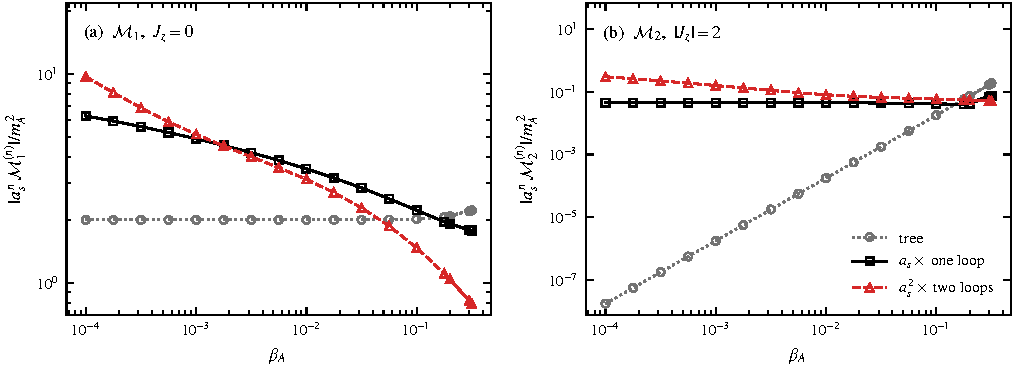
\includegraphics[width=0.94\textwidth]{figures/fig5_amplitudes.pdf}
 \caption{Tree-level, one-loop and two-loop terms of the Type~II amplitude, $|\as^n\mathcal M_i^{(n)}|/\mA^2$ with $\as=\BenchAs$ ($\alpha_s=\BenchAlphaS$), at $c=\BenchCos$, $\mA=\muR=\BenchMA\,\mathrm{GeV}$, $\Nc=\BenchNc$ and $\nf=\BenchNf$. Tree level: Eq.~\eqref{eq:born}; one loop: remainder of Ref.~\cite{Bhattacharya:2019bmd} with the scale dependence of Eq.~\eqref{eq:normalisation} restored; two loops: series through $\bA^6$. $\mathcal M_1$ and $\mathcal M_2$ are the equal and opposite helicity amplitudes, Eq.~\eqref{eq:helicity}.}
 \label{fig:amplitudes}
\end{figure*}


\subsection{Leading power}
\label{sec:leading}

To determine the leading threshold behaviour of the
two-loop remainders, I first collect the terms of
order $\bA^0$, including all powers of $\ln\bA$
that multiply them. The notation $\big|_{\bA^0}$ used below
denotes this part of the expansion.

In the expanded remainders, the logarithms of $\bA$ and of the angular
variables appear at leading power in the combination
$\ln\bA+\tfrac12\ln(1-c^2)$. I therefore introduce
\begin{align}
 \mathcal L
 &=\ln\bA+\tfrac12\ln(1-c^2)+\ln2+\frac{i\pi}{2}
 \nonumber\\
 &=\tfrac12\ln\bigl[-4\bA^2(1-c^2)\bigr],
 \label{eq:calL}
\end{align}
where the logarithm of the negative argument is taken on the branch
$\ln(-X)=\ln X+i\pi$ for $X>0$, which is the one followed by the remainders
in the physical region.

The meaning of $\mathcal L$ follows from Eq.~\eqref{eq:gram-scaling}.
Substituting the expressions for $tu-\mA^4$ and $p_T^2$ gives
\begin{align}
 \nonumber
 \mathcal L
 &=\tfrac12\ln\frac{\mA^4-tu}{\mA^4}
   +\ln(1-\bA^2)
 \\
 &=\ln\frac{2p_T}{\mA}+\frac{i\pi}{2}
   +\tfrac12\ln(1-\bA^2).
 \label{eq:calL-pT}
\end{align}
The last term is of order $\bA^2$. Near threshold, $\mathcal L$ is therefore
the logarithm of the transverse momentum of the pseudoscalars, up to the
constant phase $i\pi/2$ and power corrections.

When the leading power terms are rewritten in terms of $\mathcal L$, no
separate $\ln(1\pm c)$ or $\Li_2\bigl((1+c)/2\bigr)$ remains, and the
rational dependence on $c$ cancels. All dependence on the scattering angle
is then contained in $\mathcal L$, and the coefficients of its powers are
independent of $c$. For general $\Nc$ and $\nf$,
\begin{align}
 \Mfull{1}\big|_{\bA^0}
 &=\mA^2\sum_{k=0}^{3}
   \widehat A_{1k}\,\mathcal L^k,
 \\
 \Mfull{2}\big|_{\bA^0}
 &=\mA^2\sum_{k=0}^{2}
   \widehat A_{2k}\,\mathcal L^k.
 \label{eq:leading-power}
\end{align}
The highest logarithmic coefficients are
\begin{align}
 \widehat A_{13}&=\LeadOneThree,
 &
 \widehat A_{12}&=\LeadOneTwo,
 \nonumber\\
 \widehat A_{22}&=\LeadTwoTwo,
 &
 \widehat A_{21}&=\LeadTwoOne,
 \label{eq:leading-coefficients}
\end{align}
which do not depend on $\muR$, and
\begin{equation}
 \widehat A_{11}=\LeadOneOnePrefactor\bigl(\Nc\,a_{\mathrm{A}}-\nf\,a_{\mathrm{F}}\bigr),
 \label{eq:M1-L1}
\end{equation}
where
\begin{align}
 a_{\mathrm{A}}&=\LeadOneOneNc,
 \nonumber\\
 a_{\mathrm{F}}&=\LeadOneOneNf,
 \nonumber
\end{align}
and $L_\mu=\ln(\mA^2/\muR^2)$. Table~\ref{tab:leading-log-benchmark} gives all coefficients for $\Nc=\BenchNc$, $\nf=\BenchNf$ and $\muR=\mA$. At $\bA^2$, $\bA^4$ and $\bA^6$ the same substitution again removes every $\ln(1\pm c)$ and $\Li_2$; the remaining dependence on the angle is rational, even in $c$ and free of poles at $c=\pm1$.


Up to the constant $i\pi/2$ and power corrections, $\mathcal L$ is the logarithm of the transverse momentum of the pseudoscalars or, equivalently, of the Gram determinant $tu-\mA^4$. The exact one-loop remainders already contain it, since they depend on
\begin{align*}
 &\ln(y-x)+\ln(z-x) \text{ and }\\
 &(y-x)(z-x)=yz-1=(tu-\mA^4)/\mA^4
\end{align*}
by Eq.~\eqref{eq:xyz-definition}. The two-loop coefficients have no finite limit as $\bA\to0$; they grow as $\mathcal L^3$ and $\mathcal L^2$.

\subsection{One loop}
\label{sec:one-loop}

Fitting the Ref.\ \cite{Bhattacharya:2019bmd} one-loop remainders at $\bA=$ \OneLoopFitBetas{} with \OneLoopDigits-digit arithmetic, for $\Nc=$ \OneLoopScanNc, $\nf=$ \OneLoopScanNf{}, two values of $\muR$ and several angles, I find to \OneLoopAgreementDigits{} digits
\begin{align}
 \mathcal M_1^{(1)}&=\mA^2\bigl[\OneLoopAone\,\mathcal L+\widehat A^{(1)}_{10}\bigr]+\Ord(\bA),
 \nonumber\\
 \mathcal M_2^{(1)}&=\OneLoopMtwo\,\mA^2+\Ord(\bA),
 \label{eq:one-loop-threshold}
\end{align}
with $\widehat A^{(1)}_{10}=\OneLoopAzero$ for $\Nc=\BenchNc$, $\nf=\BenchNf$ and $\muR=\mA$, in the normalisation of Eq.~\eqref{eq:normalisation}. The constant does not depend on the angle, and by Eq.~\eqref{eq:normalisation}, its scale dependence is $\partial\widehat A^{(1)}_{10}/\partial\ln\muR^2=4i\beta_0$. The coefficient of $\mathcal L$ and the limit of $\mathcal M_2^{(1)}$ depend neither on $\nf$ nor on $\muR$. Together with Eqs.~\eqref{eq:born} and \eqref{eq:leading-power}, the behaviour at threshold is summarised in Table~\ref{tab:orders}.
%
\begin{table}[t]
 \caption{Behaviour of the Type~II coefficients at threshold, $\bA\to0$ at fixed angle: tree-level values, and the highest power of $\mathcal L$ at one and two loops.}
 \label{tab:orders}
 \begin{ruledtabular}
 \begin{tabular}{lccc}
  & tree level & one loop & two loops \\
  \hline
  $\mathcal M_1$ ($J_z=0$) & $2i\mA^2$ & $\mathcal L$ & $\mathcal L^3$\\
  $\mathcal M_2$ ($|J_z|=2$) & $2i\mA^2\bA^2(1-c^2)$ & $\mathcal L^0$ & $\mathcal L^2$
 \end{tabular}
 \end{ruledtabular}
\end{table}
%
The $|J_z|=2$ amplitude is suppressed near threshold only at tree level. According to Eq.~\eqref{eq:helicity}, $\mathcal A_{\pm\mp}$ retains the azimuthal factor $e^{\pm2i\phi}$ as $|\vec p_3|\to0$. The loop amplitude therefore has a direction-dependent limit and is not analytic in $\vec p_3$ at the origin. At one loop $\mathcal M_2$ approaches a nonzero constant without a DPS logarithm; at two loops it also acquires the logarithm discussed in Sec.~\ref{sec:two-loop}.

\subsection{The double parton scattering singularity}
\label{sec:dps}

\paragraph{Origin of the logarithm.}

The logarithm $\mathcal L$ in Eq.~\eqref{eq:one-loop-threshold} can be
understood from the one-loop Type~II diagrams near $p_T=0$, shown in
Fig.~\ref{fig:diagrams}(b). As $p_T\to0$, all four internal gluons can be
on shell simultaneously, two of them collinear to each incoming gluon. This
configuration is the pinch that produces the DPS singularity of the crossed
box~\cite{GauntStirling2011}.
%
The singular contribution can be expressed as
an integral over transverse momentum of the
product of the light cone wavefunctions of the
two incoming gluons and the tree amplitudes of
the two hard subprocesses~\cite{GauntStirling2011}.
The wavefunctions describe the splitting of each
incoming parton. The hard subprocess amplitudes
are evaluated with collinear on-shell incoming
partons and zero transverse momentum. Thus, the
splittings determine the strength of the
singularity, while the hard subprocesses enter
its coefficient. In the present case, the
splittings are $g\to gg$ and the subprocesses
are $gg\to A$ through $O_G$.

For a gluon splitting into a collinear pair,
the daughter helicities add to $0$ or $\pm2$,
whereas the parent helicity is $\pm1$.
The numerator of the splitting vertex therefore
vanishes in the exactly collinear limit; for the
allowed tree helicity configurations it
is linear in the relative transverse momentum.
After including the propagator, the corresponding
light cone wavefunction behaves as the inverse
of that momentum. The transverse momentum
integral is consequently at most logarithmically
singular, as in the massless quark examples
of Ref.~\cite{GauntStirling2011}.

\paragraph{Helicity selection and weights.}

The logarithm is present only for certain helicities of the partons in the
singular configuration. For the fermion loops of
Ref.~\cite{GauntStirling2011}, helicity conservation forces the four
intermediate partons into $J_z=0$; for gluon loops only conservation of
$J_z$ between the incoming state and the intermediate partons
remains~\cite{DixonEsterlis2016}. Here the effective vertices restore the
restriction. The amplitude for $gg\to A$ vanishes unless the two gluons
have equal helicities, and the gluons of each fusing pair move in opposite
beam directions, so each pair has $J_z=0$. A DPS logarithm is therefore
possible only for incoming gluons with $J_z=0$, which is why
$\mathcal M_1$ has a logarithm at one loop and $\mathcal M_2$ does not.

For a positive-helicity gluon splitting into gluons $a$ and $b$ with
longitudinal momentum fractions $z$ and $1-z$, the longitudinal weights,
up to coupling, colour and transverse momentum factors, are
\begin{align}
 w_{++}(z)&=\frac{1}{\sqrt{z(1-z)}},
 \nonumber\\
 w_{+-}(z)&=\frac{z^2}{\sqrt{z(1-z)}},
\nonumber\\
 w_{-+}(z)&=\frac{(1-z)^2}{\sqrt{z(1-z)}},
 \label{eq:splitting-weights}
\end{align}
where the subscripts give $(h_a,h_b)$~\cite{Mangano:1990by,Dixon:1996wi}.
The sum of their squares, $[1+z^4+(1-z)^4]/[z(1-z)]$, is the $z$
dependence of the $g\to gg$ splitting function. At the DPS point, the first
pseudoscalar receives a fraction $x$ of the first incoming momentum and,
since the two pseudoscalars have equal masses, a fraction $1-x$ of the
second~\cite{GauntStirling2011}; in Fig.~\ref{fig:diagrams}(b),
$k=xp_1$ and $p_3-k=(1-x)p_2$. Here $x$ and $z$ are momentum fractions,
not the variables of Eq.~\eqref{eq:xyz-definition}.

Since $A$ is odd under parity, which reverses all helicities, the
amplitudes for $g^+g^+\to A$ and $g^-g^-\to A$ have opposite
signs~\cite{Dixon:1996wi}. For two incoming positive-helicity gluons, with
the first helicity of each daughter pair referring to the gluon that goes
to the first pseudoscalar, each vertex requires equal helicities, so both
splittings produce the same pair: $(+,+)$, $(+,-)$ or $(-,+)$. In the mixed
cases one vertex receives two negative-helicity gluons, and these
contributions enter with the opposite sign. The factorised form of
Ref.~\cite{GauntStirling2011} then gives
\begin{align}
 F_A(x)
 &=w_{++}(x)w_{++}(1-x)
 \nonumber\\
 &\quad-w_{+-}(x)w_{+-}(1-x)
       -w_{-+}(x)w_{-+}(1-x)
 \nonumber\\
 &=\frac{1}{x(1-x)}-2x(1-x),
 \label{eq:FA}
\end{align}
since each mixed product equals $x(1-x)$. For a CP-even coupling to $G^2$
the two signs are equal and the mixed terms add:
\begin{equation}
 F_S(x)=\frac{1}{x(1-x)}+2x(1-x).
 \label{eq:FS}
\end{equation}
These weights differ from those of the massless quark boxes for
$gg\to HH$ in Ref.~\cite{GauntStirling2011}, where internal quarks of equal
helicity carry complementary momentum fractions and the weight is
proportional to $x(1-x)$.

\paragraph{Normalisation and the forward limit.}

At threshold, both pseudoscalars are at rest
and $x=\tfrac12$, so that
$F_A(\tfrac12)=\tfrac72$ and
$F_S(\tfrac12)=\tfrac92$.
By Eq.~\eqref{eq:calL}, the coefficient of
$\ln p_T^2$ is half the coefficient of
$\mathcal L$. The one-loop threshold result
in Eq.~\eqref{eq:one-loop-threshold}
therefore gives
\[
 \frac{\OneLoopAone\,\mA^2}{2}
 =\frac72\pi\Nc\mA^2
 =\pi\Nc\mA^2F_A\!\left(\frac12\right).
\]
Matching at threshold thus fixes the overall
factor multiplying $F_A$ to $\pi\Nc\mA^2$.
This factor is obtained from the calculated
amplitude; it has not been derived independently
from the factorisation formula.

Having fixed this constant, the predicted
dependence on $x$ can be tested away from
threshold. The forward limit $c\to1$ at
fixed velocity also gives $p_T\to0$, but the
produced bosons now move along the beam.
Since the test is also applied to $gg\to HH$ later, I denote the velocity and mass of the produced bosons by $\beta$ and $m$, with $\beta=\bA$ and $m=\mA$ for $AA$.
In this limit, the longitudinal velocity of
the first boson is $2x-1$, so
$x=(1+\beta)/2$.

To extract the logarithmic coefficient, I
differentiate the real part of the one-loop
remainder with respect to $\ln p_T^2$ at
fixed $\beta$ and $m$, and then take the
forward limit. Dividing by the normalisation
fixed above defines
\begin{align}
 D(\beta)
 &\equiv
 \frac{1}{\pi\Nc m^2}
 \lim_{c\to1}
 \frac{\partial\,\Real\mathcal M_1^{(1)}}
      {\partial\ln p_T^2}
 \nonumber\\
 &=F_A\!\left(\frac{1+\beta}{2}\right)
 \qquad (gg\to AA).
 \label{eq:dps-prediction}
\end{align}
The last equality is the prediction to be
tested: no further adjustment of the
normalisation is made as $\beta$ is varied.
%
I evaluated $D(\beta)$ from the exact one-loop
remainders using $1-c=10^{-14}$ and
$10^{-18}$, over
$\DPSBetaMin\leq\beta\leq\DPSBetaMax$,
with $\Nc=$ \DPSNcValues{} and
$\nf=$ \DPSNfValues{}.
The largest relative deviation from
Eq.~\eqref{eq:dps-prediction} was
\DPSMaxDeviation{}.
The extracted coefficients follow the
pseudoscalar weight $F_A$, rather than
the scalar weight $F_S$, over the tested
range.

\paragraph{Comparison with scalar pair production.}

The scalar process provides a separate test
of the relative signs in the helicity sum.
The splittings and colour factors are
unchanged, while replacing the CP-odd
vertices by CP-even ones changes $F_A$
to $F_S$.
I tested this prediction using the one-loop amplitudes for $gg\to HH$ in which each scalar is emitted from its own effective vertex, at the same mass $m$. I computed them with the code of Ref.~\cite{Bhattacharya:2019bmd}, replacing the CP-odd vertices of $O_G$ by those of the CP-even operator $H\,G^a_{\mu\nu}G^{a\mu\nu}$ and leaving the rest of the calculation unchanged.
The code reproduces the one-loop $AA$
result of that reference to
\HHReproduceDigits{} digits, and the
$HH$ double poles agree with Catani's
formula~\cite{Catani:1998bh}.

In the conventions used here, the $HH$
tree amplitude at threshold is $-2im^2$,
opposite in sign to the $AA$ amplitude.
The corresponding forward coefficient
satisfies
\[
 D(\beta)
 =-F_S\!\left(\frac{1+\beta}{2}\right)
 \qquad (gg\to HH)
\]
to a relative accuracy of \HHDpsMaxDev{}
for $\HHBetaMin\leq\beta\leq\HHBetaMax$.
The normalisation fixed from $AA$ therefore
also reproduces the $HH$ logarithm without
an additional fitted constant. In units
of the respective tree amplitudes, the
ratio of the scalar and pseudoscalar
logarithmic coefficients at threshold is
\begin{equation}
 \dfrac{F_S(\tfrac12)}{F_A(\tfrac12)} = \dfrac{9}{7}.
\end{equation}
%$F_S(\tfrac12)/F_A(\tfrac12)=\tfrac97$.

The opposite helicity amplitude again
has no logarithm. Its extracted forward
coefficient is about \HHMtwoMax{} times
that of $\mathcal M_1$.
For this check, the diagram containing
the four-gluon term of the CP-even
operator and the contact counterterm
for two such insertions were not
included. Neither depends on $p_T$,
so neither changes the logarithmic
coefficient being tested.

Figure~\ref{fig:dps}(a) compares the extracted coefficients with the two helicity weights. The $AA$ points for $(\Nc,\nf)=(3,5)$ and $(4,2)$ lie on top of each other and on the curve $F_A$, so that after the normalisation of Eq.~\eqref{eq:dps-prediction} the coefficient does not depend on $\Nc$ or $\nf$. The $HH$ points (triangles), plotted with their sign reversed, lie on the curve $F_S$, which is separated from $F_A$ by
\begin{equation}
 F_S-F_A=4x(1-x)=1-\beta^2.
\end{equation}
Panel~(b) shows the relative deviations from the prediction, at most \DPSMaxDeviation{} for $AA$ and \HHDpsMaxDev{} for $HH$; the two-loop points are discussed in Sec.~\ref{sec:two-loop}.
%
\begin{figure}[!htb]
 \centering
 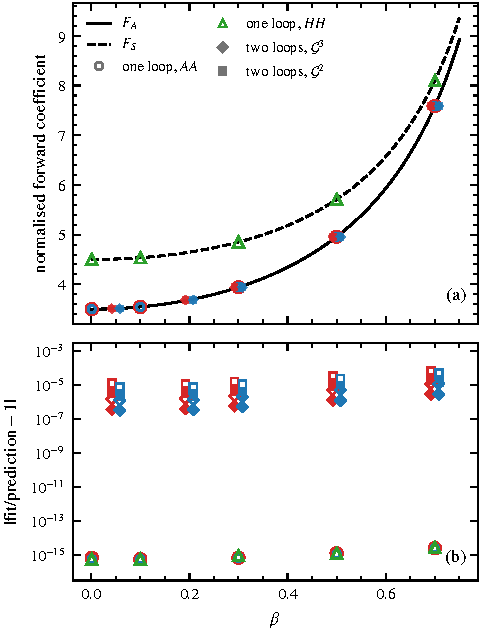
\includegraphics[width=\columnwidth]{figures/fig7_dps.pdf}
 \caption{Forward coefficients and helicity weights. (a) Circles: $D(\beta)$ for $gg\to AA$, Eq.~\eqref{eq:dps-prediction}, for $(\Nc,\nf)=(3,5)$ (red, large) and $(4,2)$ (blue, small), which coincide. Triangles: $-D(\beta)$ for $gg\to HH$ through two CP-even effective vertices at $(\Nc,\nf)=(3,5)$; the sign reversal accounts for the relative sign of the scalar and pseudoscalar tree amplitudes at threshold. Filled diamonds and squares: the coefficients of $\mathcal G^3$ and $\mathcal G^2$ in the forward limit of the two-loop remainder of $gg\to AA$, divided by $-\tfrac43\Nc\cdot2\pi\Nc m^2$ and $-2\beta_0\cdot2\pi\Nc m^2$ (Sec.~\ref{sec:two-loop}), for the same two sets (red and blue, drawn side by side). Solid and dashed curves: $F_A((1+\beta)/2)$ and $F_S((1+\beta)/2)$. (b) Relative deviations from these predictions; for the two-loop coefficients, filled symbols are fits over $1-c=10^{-7},\ldots,10^{-10}$ and open symbols include $1-c=10^{-6}$.}
 \label{fig:dps}
\end{figure}

\paragraph{Colour, scale dependence and phase.}

The factorisation also explains the flavour
and colour dependence of the one-loop
logarithm. The $O_G$ vertices couple only
to gluons, so only gluon splittings enter this
singular configuration and its coefficient is
independent of $\nf$. The factor $\Nc$
comes from the colour contraction of
the two three-gluon vertices.
Renormalisation and IR subtraction
do not change this logarithmic coefficient:
at one loop, their contributions are
proportional to the tree amplitude and
do not generate a logarithm of $p_T$.
The coefficient is therefore independent
of $\muR$.

Finally, the coefficient
$\OneLoopAone\,\mA^2$ of $\mathcal L$ is
real, whereas
$\mathcal M_1^{(0)}\to2i\mA^2$
at threshold. The logarithm is thus
out of phase with the tree amplitude
by $90^\circ$.
This relative phase is consistent
with the absorptive origin of the
one-loop DPS singularity, which can
be obtained from cuts that put
internal lines on
shell~\cite{GauntStirling2011}.
It explains why the one-loop DPS
logarithm does not contribute to
the interference with the tree
amplitude, as discussed in
Sec.~\ref{sec:rate}.

\subsection{Two loops}
\label{sec:two-loop}

The leading logarithms of the calculated two-loop coefficient $\mathcal M_1$ can be written in terms of the one-loop DPS logarithm. Comparing the coefficients of Eq.~\eqref{eq:leading-coefficients} with the coefficient $\OneLoopAone$ of Eq.~\eqref{eq:one-loop-threshold} gives, for general $\Nc$ and $\nf$,
\begin{equation}
 \widehat A_{13}\mathcal L^3+\widehat A_{12}\mathcal L^2
 =\OneLoopAone\,\mathcal L\left[\LogRelationCubic\,\mathcal L^2-2\beta_0\,\mathcal L\right],
 \label{eq:log-relation}
\end{equation}
with $\beta_0$ as in Eq.~\eqref{eq:normalisation}.
A similar relation holds in planar $\mathcal N=4$ super Yang--Mills theory.
Reference~\cite{DixonEsterlis2016} studied the six-gluon maximally
helicity violating (MHV) amplitude in planar $\mathcal N=4$ super
Yang--Mills theory, which has two negative and four positive helicities
when all momenta are outgoing. Near the configuration that mimics double
parton scattering, its singular terms obey an evolution equation, derived
following the analysis of crossing Wilson lines by Korchemskaya and
Korchemsky~\cite{KorchemskayaKorchemsky1995}, which fixes the leading
logarithms to all orders. The ratio of the leading two-loop and one-loop
terms, including their powers of the coupling, is $-(a/6)\ln^2\delta$,
where $a=g^2\Nc/(8\pi^2)$ and $\delta$, which measures the approach to the
singular configuration, is proportional to the squared transverse momentum
at fixed values of the other kinematic variables. With $a=2\Nc\as$ and
$\ln\delta=2\mathcal L+\mathrm{const}$, the ratio becomes
$-\tfrac43\Nc\as\mathcal L^2$ at leading logarithmic order. This is the
ratio of the cubic term in Eq.~\eqref{eq:log-relation} to the one-loop
logarithm, once the additional power of $\as$ at two loops is included.
The second term, $-2\beta_0\mathcal L$, has no counterpart in the
$\mathcal N=4$ theory; the number of quark
flavours enters it only through $\beta_0$.


The same $\beta_0$ term appears in the NLO momentum-space kernel for the
splitting $g\to gg$ in unpolarised colour singlet double parton
distributions~\cite{Diehl:2019rdh}, in which the transverse momentum
mismatch $\Delta$ between amplitude and conjugate amplitude plays the role
of $p_T$. Equations~(50) and (135) of Ref.~\cite{Diehl:2019rdh} give the
coefficient of $\ln^2(\mu^2/\Delta^2)$ in units of $\alpha_s/2\pi$;
relative to the LO term, its $\beta_0$ part corresponds to
$-2\beta_0\mathcal L$ in the normalisation of $\as$ used here. Half of it
comes from the renormalisation of the coupling and half from the
$\delta$-function parts of the DGLAP kernels, so that the running of the
coupling alone would give $-\beta_0\mathcal L$. The other terms of the
kernel have no counterpart in the amplitude: a term proportional to
$C_A\ln[x(1-x)]$ from the plus distributions, which contributes where the
two momentum fractions add up to one, and the real emission terms, which
contribute where they add up to less than one.


The relation of Eq.~\eqref{eq:log-relation} is not restricted to threshold. In the forward limit at fixed velocity a convenient variable is $\mathcal G=\tfrac12\ln[(\mA^4-tu)/\mA^4]=\mathcal L-\ln(1-\bA^2)$, in which the one-loop DPS logarithm is $C_1\mathcal G$ with $C_1=2\pi\Nc m^2F_A\bigl((1+\beta)/2\bigr)$, by Eq.~\eqref{eq:dps-prediction}. In this limit the two-loop logarithms of the threshold series are exactly $C_1\bigl[-\tfrac43\Nc\,\mathcal G^3-2\beta_0\,\mathcal G^2\bigr]$ through $\bA^6$, for general $\Nc$ and $\nf$; at fixed angle, the coefficient of $\mathcal L^3$ follows the expansion of $F_A\bigl((1+\bA)/2\bigr)$ order by order. Away from threshold I evaluated the released two-loop remainder of $\mathcal M_1$ at $1-c=10^{-6},\ldots,10^{-10}$ with \MoneFwdDigits-digit arithmetic, checked with \MoneFwdCheckDigits{} digits, which agree to at least \MoneFwdCheckAgreement{} digits, and fitted a cubic polynomial in $\ln(1-c)$. For $\MoneFwdBetaMin\leq\beta\leq\MoneFwdBetaMax$ and $(\Nc,\nf)=$ \MoneFwdSets, the coefficients of $\mathcal G^3$ and $\mathcal G^2$ agree with this form to \MoneFwdDevThree{} and \MoneFwdDevTwo{}, with imaginary parts below \MoneFwdImag{} of their magnitudes, when the point at $1-c=10^{-6}$ is left out; with it, the deviations are about \MoneFwdWindowFactor{} times larger, as expected from power corrections in $1-c$ (Fig.~\ref{fig:dps}). In the forward limit, the two-loop leading logarithms of $\mathcal M_1$ are therefore the one-loop DPS logarithm, with its helicity weight $F_A(x)$, multiplied by the same factor at every velocity tested.

The $|J_z|=2$ amplitude acquires a logarithm at two loops: the term
$\widehat A_{22}\mathcal L^2$, with
$\widehat A_{22}=(\MtwoRelation)\cdot\OneLoopMtwo$, is the one-loop
constant multiplied by $\MtwoRelation\,\mathcal L^2$. The forward-limit calculation described next indicates that the same coefficient relation persists away from threshold. In the forward limit $c\to1$ at fixed velocity, where $p_T\to0$ as well, I evaluated the released two-loop remainder of $\mathcal M_2$ at $1-c=$ \JzExponents{} with \JzDigits-digit arithmetic and fitted a quadratic polynomial in $\ln(1-c)$; a repetition with \JzCheckDigits{} digits agrees to at least \JzCheckAgreement{} digits. For $\JzBetaMin\leq\beta\leq\JzBetaMax$ and $(\Nc,\nf)=$ \JzSets, the real part of the coefficient of $\ln^2(2p_T/m)$ equals $-4\Nc$ times the forward limit of $\mathcal M_2^{(1)}$ to \JzMaxDev, although that limit varies by a factor of \JzKOneRatio{} over this range. Its imaginary part, which should vanish, is below \JzImag{} of its magnitude, and including the point at $1-c=10^{-4}$ in the fit increases the deviation to \JzMaxDevWide, as expected from power corrections. Within the range tested, the one-loop amplitude and the fitted two-loop logarithm are therefore consistent with
\begin{equation}
 \as\mathcal M_2^{(1)}\bigl[1-4\Nc\as\ln^2(2p_T/m)\bigr],
 \label{eq:jz2-forward}
\end{equation}
with no additional velocity or flavour dependence resolved in the coefficient of the double logarithm.


The observed combination has the form of the expansion of
$\exp(-4\Nc\as\mathcal L^2)$ to first order in $\as$. Multiplied by the one-loop coefficient $\OneLoopAone$ and
integrated over $\mathcal L$, the same exponential gives the cubic term of
Eq.~\eqref{eq:log-relation}. At lowest order it also corresponds to the
factor $\exp(-\gamma_K\ln^2\delta/8)$ of Ref.~\cite{DixonEsterlis2016},
with the cusp anomalous dimension $\gamma_K=4a$. However, two loops cannot
decide whether this factor exponentiates in QCD. The $J_z$ argument of
Sec.~\ref{sec:dps} concerns the one-loop singularity and does not forbid
this logarithm. Nor can it come from two-loop amplitudes of the
subprocesses, since conservation of angular momentum forbids $gg\to A$ for
opposite gluon helicities to all orders; its dynamical origin remains open. A related
effect occurs in planar $\mathcal N=4$ super Yang--Mills theory. The
next-to-MHV (NMHV) six-gluon amplitude, with three negative helicities, has
no such singularity at one loop because of $J_z$ conservation, but Dixon
and Esterlis found logarithmic singularities starting at two loops, in the
region where the limit overlaps with multi-Regge kinematics, and suggested
that they may come from contributions in which more than one particle
crosses a cut~\cite{DixonEsterlis2016}.

The forward limit of $\mathcal M_2^{(1)}$ itself has a closed form. The exact one-loop remainders agree with
\begin{equation}
 \lim_{c\to1}\frac{\mathcal M_2^{(1)}}{m^2}=\pi\Nc\,\frac{x^4+(1-x)^4}{x(1-x)},\qquad x=\frac{1+\beta}{2},
 \label{eq:K1}
\end{equation}
to \KOneClosedDev{} for $\KOneBetaMin\leq\beta\leq\KOneBetaMax$ and both sets of $(\Nc,\nf)$; at threshold it gives $\OneLoopMtwo$. With the weights of Eq.~\eqref{eq:splitting-weights}, the fraction in Eq.~\eqref{eq:K1} equals $w_{+-}(x)w_{-+}(1-x)+w_{-+}(x)w_{+-}(1-x)$: the helicity sum of Sec.~\ref{sec:dps} for the two pairings that an opposite-helicity initial state allows when each effective vertex receives two gluons of equal helicity, with the same overall factor $\pi\Nc$ as in Eq.~\eqref{eq:dps-prediction}. The one-loop constant of $\mathcal M_2$ thus has the form expected if it arose from the DPS region, where the azimuthal phase of these pairings removes the logarithm and leaves a finite term; I have not derived this from the factorisation formula. The two helicity amplitudes therefore provide an explicit two-loop QCD benchmark for a more general description of this singular kinematic region.


%
Figure~\ref{fig:amplitudes} compares the three orders. With $\as=\BenchAs$ ($\alpha_s=\BenchAlphaS$), at $\bA=\LoopSizeBeta$ and $c=\BenchCos$, the one and two-loop terms of $\mathcal M_1$ are \MoneOneLoopRatio{} and \MoneTwoLoopRatio{} times the tree term, and the one-loop term of $\mathcal M_2$ is \MtwoOneLoopRatio{} times the tree term. The last ratio grows as $\bA^{-2}$ towards threshold, since the tree-level $|J_z|=2$ amplitude vanishes there. The one-loop terms include the scale term of Eq.~\eqref{eq:normalisation}. Towards threshold, the loop terms of $\mathcal M_1$ grow with $|\mathcal L|$, the two-loop term as $|\mathcal L|^3$ and the one-loop term as $|\mathcal L|$, so that below $\bA\approx\CrossoverBeta$ the two-loop term exceeds the one-loop term at this angle. Because the logarithms are out of phase with the tree amplitude, this growth largely drops out of the cross section (Sec.~\ref{sec:rate}). In panel (b) the one-loop term of $\mathcal M_2$ tends to the constant of Eq.~\eqref{eq:one-loop-threshold}, while the two-loop term grows as $\mathcal L^2$, the logarithm that the $|J_z|=2$ amplitude acquires at two loops.
%
